\section{Zielsetzung}
\label{sec:Zielsetzung}

In diesem Versuch soll mittels Tomographie die Materialzusammensetzung eines Würfels
bestimmt werden. Dafür wird der Würfel zunächst mit Gammaquanten bestrahlt, 
während hinter ihm die Intensität der nicht absorbierten Strahlung gemessen werden 
kann. Dann kann durch Abgleich mit bekannten Absorptionskoeffizienten das Material bestimmt
werden.

\section{Theorie}
\label{sec:Theorie}

Das hier verwendete Verfahren der Tomographie bezeichnet allgemein die räumliche Darstellung 
eines Körpers durch Schnittbilder bzw. Projektionen. In diesem Versuch kann eine 
Tomographie realisiert werden, indem das zu untersuchende Material mit Gammaquanten 
bestrahlt wird. Dabei treten Wechselwirkungen zwischen der Strahlung und Materie auf, 
sodass nur ein Teil der Strahlung hinter dem Medium detektiert werden kann. 
Der absorbierte Strahlungsanteil ist materialspezifisch und kann über einen entsprechenden
Absorptionskoeffizienten bestimmt werden.

\subsection{Strahlungsintensität}

Die verwendeten Gammastrahlen werden durch eine $\ce{137^55_Cs}$-Quelle emittiert. 
Dabei zerfällt $\ce{137^55_Cs}$ zunächst über einen $\beta^-$-Zerfall in  $\ce{137^56_Ba}$.
94,6 \% des entstandenen $\ce{137^56_Ba}$ befinden sich in einem instabilen, angeregten 
Zustand und emittieren ein Photon mit einer Energie von $\SI{662}{\kilo\eV}$, welches 
somit als Gammaquant bezeichnet werden kann. 
Der beschriebene Zerfall ist in der folgenden Abbildung dargestellt.

\begin{figure}
	\centering
	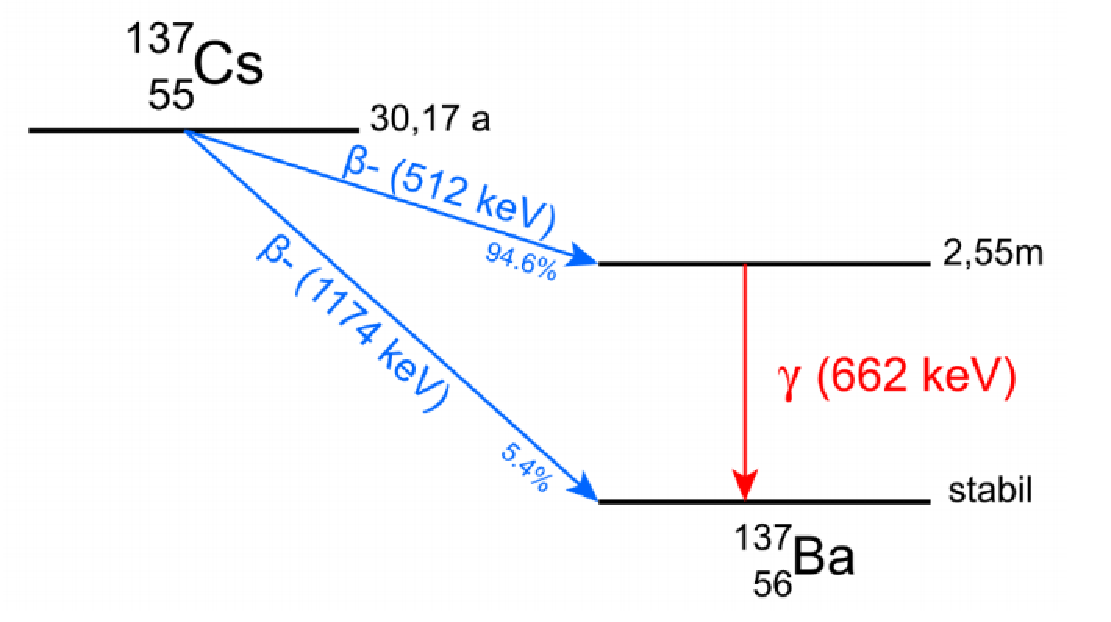
\includegraphics[width=0.8\textwidth]{figure/Zerfall.pdf}
	\caption{In dieser Abbildung ist die Entstehung der verwendeten Gammastrahlung
	schematisch dargestellt \cite{1}.} 
	\label{abb1}
\end{figure}

Trifft die beschriebene Strahlung auf Materie kann sie über den Photoeffekt oder den 
Comptoneffekt wechselwirken. Paarbildung ist erst ab einer Photonenenergie von 
$\SI{1}{\mega\eV}$ möglich, weil mindestens die Ruheenergie eines Elektrons und eines 
Positrons erreicht werden muss und daher in diesem Fall irrelevant.
Beim Photoeffekt kann die gesamte Photonenenergie in der Materie deponniert werden
(im Spektrum als Photopeak erkennbar), 
da sie an ein Hüllenelektron übertragen wird, welches daraufhin mit einer 
entsprechenden kinetischen Energie frei werden kann. Das bedeutet die Energie des Photons 
muss mindestens die Höhe der Bindungsenergie des ELektrons haben, um diese Form der 
Wechselwirkung durchzuführen. Bis zu einer Energie von $\SI{100}{\kilo\eV}$ dominiert 
der Photoeffekt, sodass in diesem Fall eher der Comptoneffekt als Primärwechselwirkung überwiegt.
Dies ist bis zu einer Energie von $\SI{1}{\mega\eV}$ der Fall. Dabei wird ein Teil der 
Photonenergie über inelastische Streuung an ein Elektron abgegeben.
Allerdings muss gesagt werden, dass ein Photon nach mehrfachem Comptoneffekt immer 
wahrscheinlicher auch einen Photoeffekt durchführt. Bei einem 
Streuwinkel von 180° findet der maximale Energieübertrag statt. Im Spektrum wird an 
dieser Stelle von der Comptonkante gesprochen. 
Die Intensitätskurve zeigt außerdem ein Plateau am Anfang, welches aufgrund von 
Rückstreueffekten entstanden ist. Die Intensität der Strahlung die 
nach Durchqueren des Materials noch vorhanden ist wird durch die Gleichung 

\begin{equation}
	I = I_0 \exp \left( \sum_i \mu_i d_i \right)
	\label{eq1}
\end{equation}

beschrieben. In dieser Gleichung beschreibt $I_0$ die Eingangsintensität und $d_i$ die 
Dicke des Materials $i$ mit dem Absorptionskoeffizienten $\mu_{i}$. Der 
Verlauf einer typischen Intensitätskurve für einen 
$\ce{137^55_Cs}$-Strahler ist in der folgenden Abbildung dargestellt \cite{Kerne}.

\begin{figure}
	\centering
	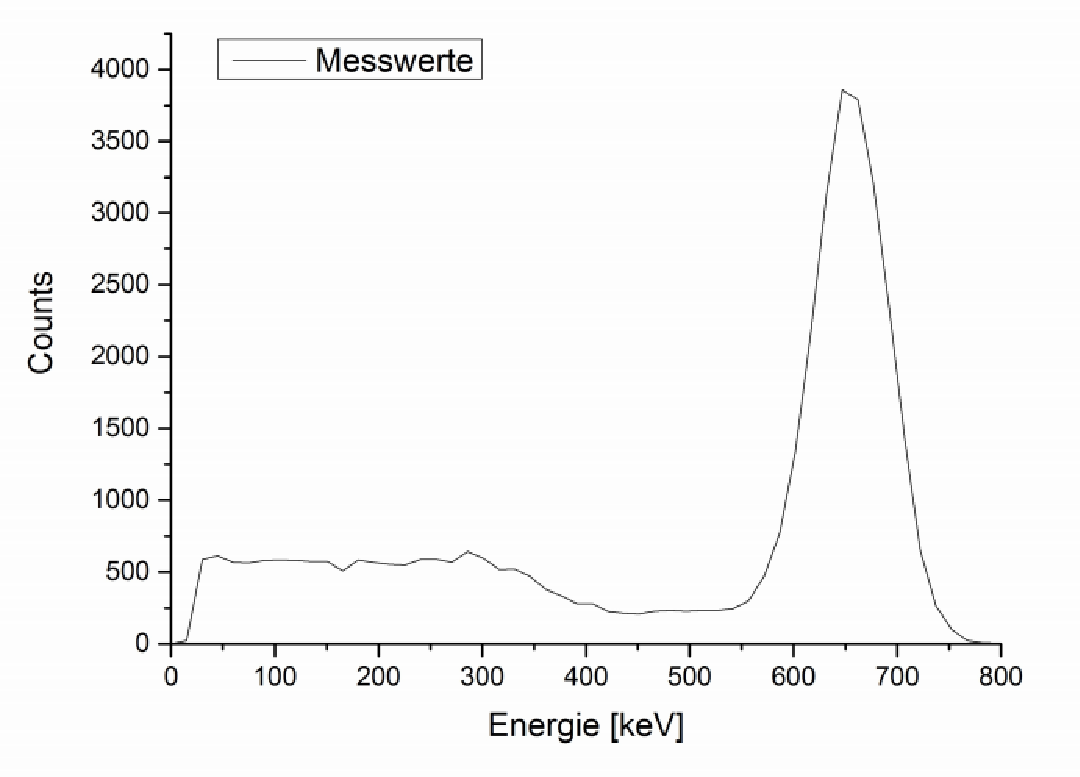
\includegraphics[width=0.7\textwidth]{figure/Kurve.pdf}
	\caption{In dieser Abbildung ist der Verlauf einer Intensitätenkurve für 
	$\ce{137^55_Cs}$ dargestellt.}
	\label{abbkurve}
\end{figure}
\FloatBarrier

\subsection{Absorptionskoeffizienten}
\label{sec:Absorp}

Die materialspezifischen Absorptionskoeffizienten können mit Gleichung \eqref{eq1} 
berechnet werden, da die Intensitäten gemessen werden und die Materialdicken bekannt sind.
Daher ergibt sich durch umformen


\begin{equation}
	\sum_i \mu_i d_i  = \ln \left( \frac{I_0}{I_j} \right)
	\label{eq2}
\end{equation}

und in Matrixschreibweise


\begin{equation}
	A \cdot \vec{\mu} = \vec{I},
	\label{eq3}
\end{equation}

wobei $A$ eine $n \times m$-Matrix ist, die die Weglängen durch bestimmte Materialien 
enthält die bei einem zugehörigen Strahlengang passiert werden. $\vec{\mu}$ enthält die 
passenden Absorptionskoeffizienten. Mit der Methode der kleinsten Quadrate kann 
mit Gleichung \eqref{eq3} der Zusammenhang 


\begin{equation}
	WA \cdot \vec{\mu} = W \vec{I}
	\label{eq4}
\end{equation}

bestimmt werden.
Hierbei entspricht $W$ einer Gewichtsmatrix


\begin{equation}
	W = V[I]^{-1},
	\label{eq5}
\end{equation}

die über die inverse Varianz der 
Intensitäten definiert ist, sodass sich für $\vec{\mu}$ schließlich die Relation 


\begin{equation}
	\vec{\mu} = (A^{T}WA)^{-1}(A^{T}W\vec{I})
	\label{eq6}
\end{equation}

ergibt und die Unsicherheiten aufgrund der Poissonfehler eines Zählexperimentes durch


\begin{equation}
	V[\mu]= (A^{T}WA)^{-1}
	\label{eq7}
\end{equation}

gegeben sind \cite{Kerne}.
\newpage

























